\documentclass{webofc}
\usepackage[varg]{txfonts}
\usepackage{natbib}

\usepackage{xcolor}

\begin{document}

\title{PanDA and RADICAL-Pilot Integration: Enabling the Pilot Paradigm on HPC Resources}

\author{
  \firstname{Pavlo} \lastname{Svirin}\inst{1} \and
  \firstname{Matteo} \lastname{Turilli}\inst{2} \and
  \firstname{Andre} \lastname{Merzky}\inst{2}
}

\institute{Brookhaven National Laboratory \and
           Rutgers University 
}

\abstract{PanDA executes millions of ATLAS jobs a month on Grid systems with
more than 300,000 cores. Currently, PanDA is compatible only with few HPC
resources due to different edge services and operational policies; does not
implement the pilot paradigm on HPC; and does not dynamically optimize
resource allocation among queues. We integrated the PanDA Harvester service
and the RADICAL-Pilot (RP) system to overcome these disadvantages and enable
the execution of ATLAS, Molecular Dynamics and other workloads on HPC
resources. Harvester is a commonality layer which brings coherence to diverse
HPC systems, providing integration with PanDA workloads at job and event
level. RP is a pilot system capable of executing short/long-running
single/many-cores tasks on diverse HPC machines, supporting CPUs, GPUs, and
multiple MPI implementations. We integrated Harvester and RP on Titan at
ORNL, prototyping a Next Generation Executor (NGE) to expose RP capabilities
and manage the execution of PanDA workloads.}

\maketitle

% ---------------------------------------------------------------------------
\section{Introduction}
\label{intro} 

PanDA is the Workload Management System (WMS) used by the ATLAS experiment at
the LHC to execute scientific applications on widely distributed resources.
PanDA is designed to support the execution of distributed workloads via pilots~\cite{turilli2018comprehensive}. Pilot-capable WMS
enable high throughput execution of tasks via multi-level scheduling while
supporting interoperability across multiple sites. This is particularly
relevant for LHC experiments, where millions of tasks are executed across
multiple sites every month, analyzing and producing petabytes of data.

The implementation of PanDA WMS consists of several interconnected
subsystems, communicating via dedicated API or HTTP messaging, and
implemented by one or more modules. Databases are used to store stateful
entities like tasks, jobs and input/output data, and to store information
about sites, resources, logs, and accounting. PanDA can execute ATLAS tasks
on a variety of infrastructures, including high performance computing
facilities. In the past three years, PanDA was used to execute … milion jobs
on Titan, a leadership-class machine managed by the Oak Ridge Leadership
Computing Facility (OLCF) at the Oak Ridge National Laboratory (ORNL).

Ref.~\cite{Doleynik2017high} describes in detail how PanDA has been deployed
on Titan. Importantly, it shows that while PanDA implements the pilot
abstraction to execute tasks on grid resources, on HPC facilities it submits
job directly to the batch system of the machine. The size and duration of
this job depends on resource availability and workload requirements. Resource
availability is polled from Titan every ten minutes via the backfill
functionality of the Moab scheduler and a job is submitted requiring the
available amount of resources. The workload of this job is sized so to allow
its execution within the available walltime. PanDA uses Titan’s resources to
execute Geant4 event simulations, a specific type of workload that is
amenable to execute via the machine’s batch system.

In this paper, we present the integration between Harvester and Next
Generation Executor (NGE). Harvester is a new resource-facing service
developed by ATLAS to enable execution of ATLAS workloads on HPC machines,
bringing further coherence in the PanDA stack across the support of different
types of infrastructures, like grid and HPC. NGE is a REST interface
developed for RADICAL-Pilot, a pilot system designed to support
high-throughput computing on HPC infrastructures, including leadership-class
machines like Titan. Different from Harvester, NGE enables to submit a pilot
job via the batch system of Titan and then directly scheduling tasks on the
acquired resources without queuing in the machine batch system. In this way,
tasks can be executed immediately while respecting the policies of the HPC
machine.

PanDA can benefit from pilot capabilities in several ways. Pilot do not
require to package a workload into a batch queue submission script,
simplifying the deployment requirement. Further, pilots enable the concurrent
and sequential execution of a number of tasks, until the available walltime
is exhausted. Concurrent because a pilot holds multiple nodes of an HPC
machine enabling the execution of multiple tasks at the same time; sequential
because when a task completes, another task can be executed on the freed
resources. In this way, tasks can be late bound to an active pilot, depending
on the current and remaining availability. This is important because, in
principle, ATLAS would not have to assign a specific portion of tasks to an
HPC machine but it could assign them only when the resources become
available. Thus this would bring further coherence to ATLAS software stack,
as pilots and late binding are already used for grid resources.

RADICAL-Pilot offers a number of distinctive features. Among these, the most
relevant for ATLAS is the possibility to run arbitrary tasks on any given
pilot. Specifically, RADICAL-Pilot decouples the management of a pilot, the
coordination of task executions on that pilot, and what each task executes.
For example, if a task executes a Geant4 simulation and another a molecular
dynamic simulation, both tasks can run at the same time on the same pilot.
Further, RADICAL-Pilot enables also the concurrent execution of different
tasks on CPU and GPU, allowing for the full utilization of HPC worker nodes
resources. This capabilities will enable PanDA to transition from a workload
management system designed specifically to support the execution of ATLAS
workloads, to a system for the execution of general purpose workloads on HPC
machines.


% ---------------------------------------------------------------------------
\section{Harvester}

\textcolor{red}{Harvester [Harvester]} is a resource-facing service developed for ATLAS
experiment at CERN since 2016 with a wide collaboration of experts.  It is
stateless with a modular design to work with different resource types and
workloads. The main objectives of Harvester are as follows: first, it should
be a common machinery for pilot provisioning on all ATLAS computing resources
on Grid. Second, it should provide a commonality layer bringing coherence to
HPC implementations. Third, it should add a capability to timely optimize CPU
allocation among various resource types to remove batch-level static
partitioning. Finally, it should integrate the PanDA system and resources
more tightly for new advanced workloads.

Figure 1. Harvester architecture

Figure 1 shows a schematic view of the Harvester architecture. Harvester is a
stateless service with a local master database and a central slave database.
The local database is used for real-time bookkeeping close to resources, and
the central database is periodically synchronized with the local database to
provide the resource information to the PanDA server. The PanDA server uses
the information together with global overview of workload distribution in
order to orchestrate behaviour of Harvester instances. Therefore,
communication between harvester and the PanDA server is bidirectional.
Harvester fetches job descriptions that have to be executed from PanDA Server
using communicator component, same component is used to report back the
status of these jobs. Harvester accesses resources through different plugins
(Figure 2) which have been developed by resource experts. When Harvester
instances run on edge nodes of HPC centers they access compute nodes through
local HPC batch systems using HPC submission plugins. Status of the batches
is tracked using monitor plugin. Input and output data are transferred with
various stager and preparator plugins which implement
Rucio~\cite{garonne2014rucio}, Globus Online~\cite{foster2011globus}  and
other data transfer clients. All of the communication between the components
is done via local database.


Figure. Modules used for PanDA-NGE interaction

In context of BigPanDA project several instances of Harvester have been
deployed on front nodes of BNL Institutional Cluster, NERSC (Cori), Titan and
Jefferson Lab clusters. They are serving experiments like ATLAS, LQCD, nEDM,
IceCube and LSST.


% ---------------------------------------------------------------------------
\section{RADICAL-Pilot and Next Generation Executor}\label{sec:rp}

RADICAL-Pilot (RP) is a pilot system which enables task-level concurrency on
a variety of infrastructures, including XSEDE HPC, Cloud and grid systems,
NARC Cheyenne, NCSA Blue Waters, and ORNL Reha, Titan and
Summit~\cite{merzky2018using}. As a pilot system, RP allows scheduling jobs
on HPC machines (or virtual machines on cloud infrastructures) to acquire
computing resources. Once these resources become available, RP schedules
tasks on them directly, i.e., without using the machine’s batch system. In
this way, tasks do not wait in the queue but execute immediately enabling
high-throughput on HPC machines. It is important to stress that RP, and pilot
systems in general, do not “game” the scheduling policies of the HPC
machines: resource acquisition is performed via the batch system and
resources remain available only for the given walltime period. Jobs waits in
the queue alongside all the other jobs and are subjected to queue, allocation
and fair-use policies of the system.
	
Among pilot systems, RP has unique capabilities and architectural properties.
RP offers concurrent execution of heterogeneous tasks on the same pilot,
supporting both CPU and GPU, more than twelve task launching methods---e.g.,
ssh, mpirun, aprun, openmpi---and all the major HPC batch systems---e.g.,
SLURM, PBS, Torque. RP can execute single or multi core tasks within a single
compute node, or across multiple nodes. RP isolates the execution of each
tasks into a dedicated process, enabling concurrent execution of
heterogeneous tasks by design. For example, RP can run a bag of 65,000
heterogeneous tasks, requiring between 1 and 384 cores, some running on CPU
cores, others on GPU, some using OpenMP other MPI. These tasks may run in
several ‘generations’, each with varying degree of concurrency and
combination of types of tasks. Further RP can concurrently manage multiple
pilots both on the same machine or submitted across a set of machines. Tasks
can be late-bound to available resources, using different scheduling
algorithms across resources and within each resource.
	
Architecturally, RP is designed following a so called ‘building blocks’
design approach~\cite{turilli2018building}. Consistently, RP is
self-sufficient, interoperable, extensible and partially composable.
Self-sufficient because RP independently implements the necessary and
sufficient set of functionalities for describing and managing pilot and task
entities; interoperable in terms of type of workload, resource, and execution
paradigm; and extensible as new properties can be added to the pilot, task
and resource descriptions, and more functionalities can be implemented for
this entities. Currently, composability is partially designed and
implemented: while the pilot-API can be used by both users and other systems
to describe one or more task-based workloads for execution, RADICAL-Pilot
requires RADICAL-SAGA to interface to HPC resources. A prototype interface to
cloud resources based on LibCloud is available and a general-purpose resource
connector component is under development.	
	
Figure~\ref{fig:rp-arch} shows RP architecture and execution model. RP
assumes a multi-task application written in Python, using the Pilot API. This
API let users to describe tasks---called compute units (CU)---and pilots
(Figure~\ref{fig:rp-arch}.1). Each task description has a set of properties,
including the name of the executable launched by RP, the type and amount of
cores this executable will need, whether it requires MPI, input files and so
on. Pilot descriptions also have a set of properties, including the endpoint
where the resource request should be submitted, the type and amount of
resources to acquire, and the walltime of these resources. The RP API
includes classes to create both pilot and unit managers to which pilot and
unit descriptions are assigned for execution. Once managed, pilots are
submitted to the indicated endpoint (Figure~\ref{fig:rp-arch}.2), and once
scheduled pilot bootstrap an agent (Figure~\ref{fig:rp-arch}.3). Unit
manager(s) schedule compute units onto available agent(s)
(Figure~\ref{fig:rp-arch}.4) and each agent uses a resource-specific executor
to run the units (Figure~\ref{fig:rp-arch}.5).

\begin{figure}
  \centering
  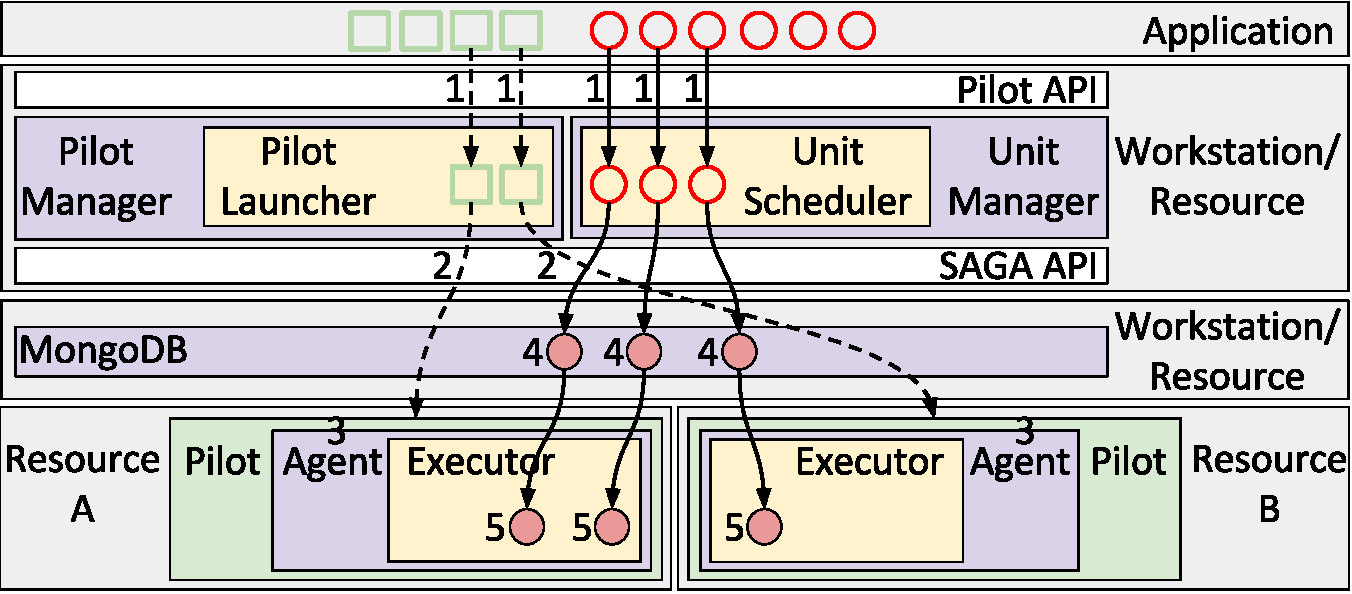
\includegraphics[width=0.49\textwidth]{figures/rp_arch.pdf}
  \caption{RADICAL-Pilot (RP) architecture and execution model.
           Architecture: interfaces (white), modules (purple), components
           (yellow), pilot entity (green), task entity called compute unit
           (red). Execution model: Pilot and units are described via the
           Pilot API (1); pilots are submitted to the indicated resource(s)
           (2); each pilot bootstraps an agent (3); compute units are
           scheduled onto available agent(s) (4) and executed
           (5).}\label{fig:rp-arch}
\end{figure}
	
Note that compute units are scheduled once the agent is active and that unit
descriptions need to be transferred from the client to the agent. This means
that the latency of each unit transfer reduces the overall utilization of the
available resources as no unit can be executed while in transit. To address
this issue, RP transfers units in bulk, reducing the overall latency of unit
transfer to a single round trip. Further, units are scheduled via a database
instance that needs to be reachable by both the machine on which the unit
managers is instantiated, and the remote machine on which the units will have
to be executed.
	
RP supports the execution of units which require staging of input and/or
output data. Units’ input and output files are managed by stager components
not represented in Figure~\ref{fig:rp-arch}. Data staging is performed
independently of the pilot lifetime, and can thus overlap with the pilot's
queue waiting time, thus reducing the impact on resource utilization.
	
The next generation executor (NGE) is a REST API that enables running RP as a
service. The REST API is a close semantic representation of the underlying
native RP API.  The service manages the lifetime of the RP unit and pilot
managers, and of the RP pilot agent, on behalf of a client. As is often the
case when translating a module or library API (which is usually invoked in a
process-local call stack) into a REST API (which is usually called over a
network link), care has to be taken to not let even moderate network
latencies impact the overall API performance.  The NGE API manages to avoid
that problem by adding support for bulk operations for those API methods most
prone to latency impacts: unit submission and state updates.
	
NGE service also provides functionality in addition to the RP API scope:
instead of requiring the client to specify pilot size, runtime and
configuration, it implements policy driven automatisms to shape a pilot based
on the received workload and on resource availability.  The service will
submit those auto-shaped pilots to the resource batch queue -- but it is also
able to inspect the target resource's backfill availability, and to shape the
pilots specifically so that they fit the available backfill constraints.
	
NGE's pilot shaping capabilities are policy driven: they can be adapted to
the configuration of the target resource, but also toward specific groups of
use cases. This makes the NGE deployments configurable for specific user
groups and projects.  In the context of the presented use case, that
configurability is used to mimic properties which were available in Panda's
native execution backends, which eases integration semantically.


% ---------------------------------------------------------------------------
\section{Integrating Harvester and NGE}

We deployed Harvester, NGE and RP, and the MongoDB instance needed by RP on
three separate containers provided by OLCF via their OpenShift service. The
container used for NGE and RP can directly submit jobs to the PBS batch
system of Titan, while the MongoDB instance can be reached by both Titan and
the NGE and RP container. This enables submission of pilot jobs to Titan and
scheduling of tasks on the resources of that pilot once scheduled and
bootstrapped.

A separate instance of Harvester has been set up in order to run experiments
of PanDA and NGE interaction (Fig. 3) on a front node of Titan supercomputer.
Because of differences in environments Harvester and NGE instances have been
installed on different nodes (data transfer node for Harvester and login node
for NGE), the communication is done via a secure tunnel between these nodes.
A special module for job submissions to NGE and job monitoring has been
developed. The functionality of these modules have been tested with dummy
jobs as well as with samples of ATLAS and \textcolor{red}{Molecular Dynamics [MD]}. Another
NGE instance that will be running in a container in OpenShift at OLCF is
under active deployment.

Figure~\ref{fig:integration} shows details of the coordination protocol
between Harvester and NGE and of the execution model of the integrated
system. RP initiates resource acquisition by submitting a configurable number
of pilots to Titan (Figure~\ref{fig:integration}.1). Once one or more pilots
become available, RP publishes the aggregate number of cores and their time
availability via NGE (Figure~\ref{fig:integration}.2). Note how NGE abstracts
the granularity of pilot resources into a resource overlay described by the
total core availability, partitioned based on the amount of time cores are
available. This partitioning is made necessary by the stacked availability of
multiple pilots on the same resource.

\begin{figure}
  \centering
  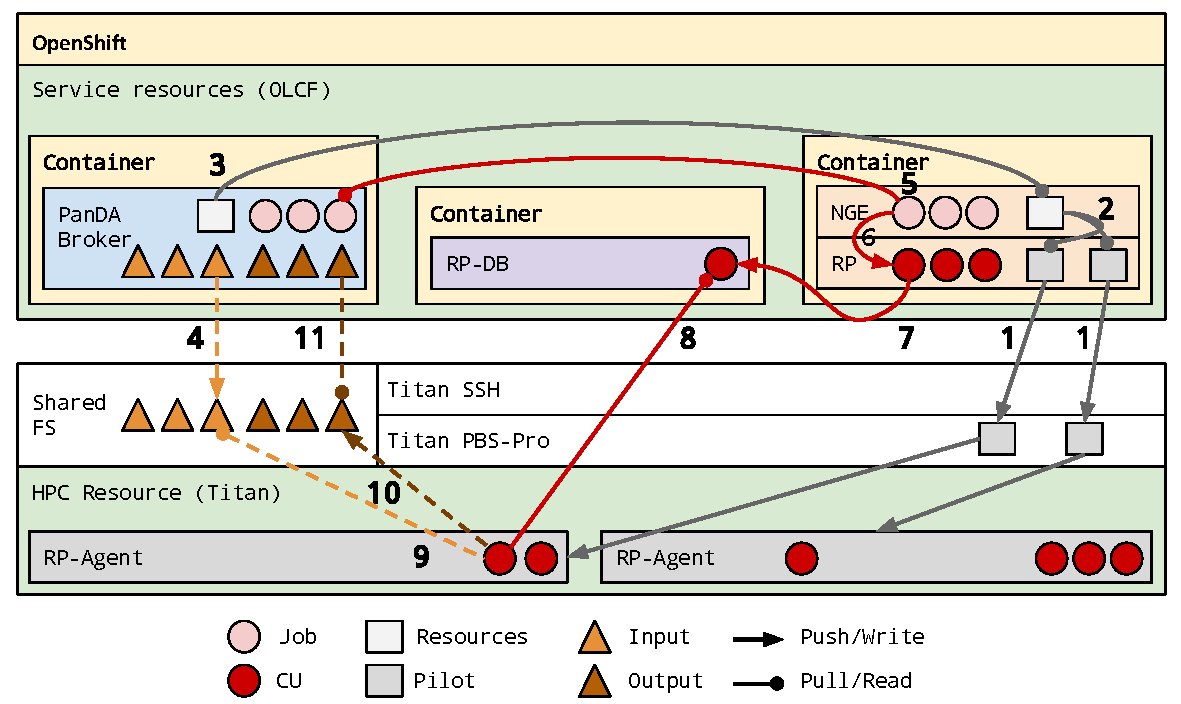
\includegraphics[width=0.49\textwidth]{figures/integration.pdf}
  \caption{Integration between Harvester and NGE deployed at OLCF to manage
           the execution of Particle Physics and Molecular Dynamics
           workloads. Harvester, NGE and RP, and MongoDB are deployed on
           containers provided and managed via
           OpenShift.}\label{fig:integration}
\end{figure}

Harvester can pull NGE to know how many cores are available and for how long
(Figure~\ref{fig:integration}.3) and push a number of tasks to NGE for
execution (Figure~\ref{fig:integration}.5). Note that before pushing tasks to
NGE, Harvester makes sure that the input data required by these tasks are
available to the work nodes of Titan. This is done by copying or linking the
relevant data to a shared file system, either local to the cluster or
available on the OLCF network (Figure~\ref{fig:integration}.5).  The number
of tasks pushed to NGE is calculate on the base of aggregated task
requirements in terms of number of cores required and walltime. Tasks are
pushed in bulk so to avoid latency and other overheads associated with
pushing single tasks. Once tasks are pushed into NGE, these are translated
into tasks descriptions for RP (Figure~\ref{fig:integration}.6) and then
executed on the available pilot resources are described in Sec.~\ref{sec:rp}
(Figure~\ref{fig:integration}.7-9). Once executed, RP stages out tasks’
output to a filesystem accessible by Harvester
(Figure~\ref{fig:integration}.10) and Harvester collects this files,
terminating the execution cycle (Figure~\ref{fig:integration}.11).

NGE can be configured to use RP to submit jobs to Titan in two modes:
standard or backfill. Standard mode supports submission of jobs to one or
more of the five PBS queues available on Titan. In this mode, job submissions
are exactly the same as any other job submitted to Titan for execution by any
other user. \textcolor{red}{In backfill mode, RP uses the … command of the Maui scheduler} to
poll the current node and walltime availability, creates a pilot description
requesting that availability and submits an equivalent job to the required
queue. In this way, RP increases the chances for that job to be immediately
scheduled on Titan, reducing the job (and therefore pilot) queue waiting
time. In this way, NGE can operate as Harvester but offering full-pilot
capabilities. This allows for Harvester to submit multiple generations of
tasks for execution on Titan, maintaining a predefined ‘pressure’ on Titan
queues. This makes the Havester/NGE integrated system execution model and
operational modality consistent across Grid and HPC, reducing the differences
in how tasks are mapped between the two types of infrastructure.


% ---------------------------------------------------------------------------
\section{Conclusions}

In this paper we introduced two distinct systems and an interface that
enabled the design and implementation of a coordination protocol for their
integration. The main contribution is to show how systems developed by two
independent teams can easily be integrated to provide new functionalities.
This suggests that end-to-end models of middleware where a single ecosystem
of modules is design to provide all the functionalities required to enable
distributed computing can be replaced by a model in which systems are
designed to be integrated. As seen in this paper, designing for integration
means developing a well-define API, making explicit the entities that can be
defined via this API and the functionalities upon these entities. Entities
and functionalities must be chosen at the right level of abstraction so to
avoid the specificity of single implementations. For example, NGE exposes
Task, Core and Walltime entities. These are sufficiently abstracted to be
consistent with both systems’ design but specific enough to define the domain
of workload management for HPC.

Currently, we deployed the integrated system at OLCF on the OpenShift
platform and we have started testing and performance characterization. As
seen in Sec. 5, the integration between NGE and RADICAL-Pilot has created no
appreciable overheads. We have now to compare the execution of a standard
ATLAS Geant4 workload with Harvester to the same execution performed with
Harverser and NGE. This comparison will measure integration overheads but
also workload execution performance. We expect that the execution on pilot
will introduce optimizations, especially related to AthenaMP setup and the
total number of events processed per walltime unit. After this
characterization, we will be ready to concurrently execute heterogeneous
workloads, using the same pilot to run tasks of distinct users from diverse
domains. This will make PanDA a general purpose workload manager and will
open the possibility to explore new resource utilization patterns on
leadership-class machines.

In this context, PanDA will leverage the design of NGE and RADICAL-Pilot to
gain access to Summit, the new leadership-class machine managed by OLCF at
ORNL. Thanks to its design, RADICAL-Pilot has been ported to Summit in less
than two months and because of the isolation between workload management and
resource acquisition, no modification of Harvester is required to execute its
workloads on Summit. As a matter of fact, Harvester will be able to execute
general purpose workloads on both Titan and Summit, at the same time and
without any modification to its code.

Following this period of testing, characterization and adoption of a new
machine, the system integrating Harvester and NGE will be evaluated for
production deployment.


% ---------------------------------------------------------------------------
% Bibliography
% ---------------------------------------------------------------------------
\bibliography{main}

\end{document}
